\documentclass[parskip,a4paper,12pt]{article}
\usepackage{tikz,pgfplots}
\pgfplotsset{temporal/.style={mark size=1pt,/pgfplots/ylabel={Amplitud},/pgfplots/xlabel={\# muestra},axis background/.style={fill=yellow!10},/pgfplots/enlargelimits=true}}
\pgfplotsset{frecuencial/.style={mark size=1pt,/pgfplots/xlabel={k (frecuencia)},/pgfplots/ylabel={Magnitud},axis background/.style={fill=blue!10},/pgfplots/enlargelimits=true}}
\usetikzlibrary{shadows.blur}
\usepackage{titletoc} %tabla de contenidos (printcontents)
\usepackage[utf8]{inputenc}
\usepackage[text={6in,9in},centering]{geometry}
\usetikzlibrary{calc,shadows,shadings}
\usepackage{lipsum}
\usepackage[spanish]{babel} %Figura en lugar de Figure
\usepackage{droidsans}
\usepackage{fancyhdr}
\usepackage{svgcolor}
\usepackage{xcolor}
\usepackage{float} %forzar ubicación de figuras
\usepackage{listings} %Código Matlab formateado
\usepackage{textcomp} %Para listings
\usepackage{amsmath} %para align
\usepackage{amssymb} %mathb
\usepackage[colorlinks]{hyperref}
\newcommand{\matlab}{\textsc{matlab}\xspace}
\usepackage{pifont} %ding
\newcommand{\flec}{\ding{224}}
\usepackage{xspace}
\usepackage{color,soul}
%%%%%%%%%%%%%%%%%%%%%%%%%%%%%%%%%%%%%%%%%%%%%%%%%%%%%%%%%%%%%%%%%%%%%%%%%%%%

%Ejercicios
%\newtheorem{ejercicio}{Ejercicio}

\usepackage{amsthm,thmtools,xcolor}
\usepackage[skins,breakable,theorems]{tcolorbox}

% \declaretheoremstyle[
%   headfont=\color{colorejercicio!50!black}\normalfont\bfseries,
%   bodyfont=\color{colorejercicio}\normalfont\itshape,
% ]{colored}

% \declaretheorem[
%   style=colored,
%   name=Ejercicio,
% ]{ejercicio}
\newtcbtheorem{enunciado}{ENUNCIADO}%
{theorem style=change apart,enhanced,arc=0mm,outer arc=0mm,breakable,theorem name and number,
boxrule=0mm,toprule=1mm,bottomrule=1mm,left=1mm,right=1mm,
titlerule=0mm,toptitle=0mm,bottomtitle=1mm,top=0mm,
colframe=colorO,colback=azulclaro!1!white,coltitle=purple,
title style={top color=white,bottom color=white,
middle color=white},
underlay unbroken and last={\draw[line width=2mm,draw=white] ($(frame.south)+(0,0.65mm)$) -- +(1.65cm,0) -- +(-1.65cm,0); \node at ($(frame.south)+(0,0.65mm)$) (){\tailpiecerule};},
fonttitle=\bfseries\sffamily\normalsize,fontupper=\normalsize\itshape, 
}{}
%%%%%%%%%%%%%%%%%%%%%%%%%%%%%%%%%%%%%%%%%%%%%%%%%%%%%%%%%%%%%%%%%%%%%%%%%%%
\usepackage{pgfornament}
\usepackage{fourier, fourier-orns}
\newcommand\tailpiecerule{\tikzset{pgfornamentstyle/.style={scale=.375}}\centerline{%\hrulefill\raisebox{-0.4ex}{~\color{NavyBlue}\decofourleft\,\decofourright~}\hrulefill
    \color{colorO}\expandafter\pgfornament\expandafter{83}}}%LightSteelBlue!50!white
%%%%%%%%%%%%%%%%%%%%%%%%%%%%%%%%%%%%%%%%%%%%%%%%%%%%%%%%%%%%%%%%%%%%%%%%%%%

% #####  Color Palette by Paletton.com
% #####  Palette URL: http://paletton.com/#uid=2370u0kllllb9vZgfqEqrg1vxaH


% *** Primary color:

%    shade 0 = #267158 = rgb( 38,113, 88) = rgba( 38,113, 88,1) = rgb0(0.149,0.443,0.345)
%    shade 1 = #6FAA96 = rgb(111,170,150) = rgba(111,170,150,1) = rgb0(0.435,0.667,0.588)
%    shade 2 = #468D76 = rgb( 70,141,118) = rgba( 70,141,118,1) = rgb0(0.275,0.553,0.463)
%    shade 3 = #0F553E = rgb( 15, 85, 62) = rgba( 15, 85, 62,1) = rgb0(0.059,0.333,0.243)
%    shade 4 = #013926 = rgb(  1, 57, 38) = rgba(  1, 57, 38,1) = rgb0(0.004,0.224,0.149)

% *** Complement color:

%    shade 0 = #AA5F39 = rgb(170, 95, 57) = rgba(170, 95, 57,1) = rgb0(0.667,0.373,0.224)
%    shade 1 = #FFC4A6 = rgb(255,196,166) = rgba(255,196,166,1) = rgb0(1,0.769,0.651)
%    shade 2 = #D48D69 = rgb(212,141,105) = rgba(212,141,105,1) = rgb0(0.831,0.553,0.412)
%    shade 3 = #803A16 = rgb(128, 58, 22) = rgba(128, 58, 22,1) = rgb0(0.502,0.227,0.086)
%    shade 4 = #551E01 = rgb( 85, 30,  1) = rgba( 85, 30,  1,1) = rgb0(0.333,0.118,0.004)

%
\definecolor{colorO}{HTML}{051F37}
%\definecolor{colorO}{rgb}{0.004,0.224,0.149}%Verde oscuro
%Negro y gris claro
\definecolor{colorB}{rgb}{0,0,0}
\colorlet{colorBFILL}{colorB!15}
%Verde 
\definecolor{colorA}{HTML}{1334A0}
%\definecolor{colorA}{rgb}{0.059,0.333,0.243}%0,0.3,0.3}
%\definecolor{colorAFILL}{rgb}{0.435,0.667,0.588}%\colorlet{colorAFILL}{colorA!10}
\colorlet{colorAFILL}{colorA!10}
\colorlet{shadecolor}{colorAFILL}
%Color complementario (crema-rojo)
\definecolor{colorC}{rgb}{0.502,0.227,0.086}%{0.5412,0.5176,0.4941}
%\definecolor{colorCFILL}{rgb}{1,0.769,0.651}%0.9098,0.8588,0.7647}
\definecolor{colorCFILL}{rgb}{0.9098,0.8588,0.7647}
%Otro verde
\definecolor{colorD}{HTML}{496A8A}
%\definecolor{colorD}{rgb}{0.149,0.443,0.345}%{0.322 ,   0.57  ,  0.563}
\colorlet{colorDFILL}{colorD!10}
%Rojo oscuro
\definecolor{colorE}{rgb}{0.333,0.118,0.004}
%\letcolor{colorE}{purple}
\definecolor{colorEFILL}{rgb}{0.831,0.553,0.412}
\colorlet{colorE}{purple}
%\colorlet{colorEFILL}{purple!10}

\tikzstyle{freecell}=[fill=colorAFILL,draw=colorA]
\tikzstyle{freestruct}=[fill=colorBFILL,draw=colorB]
\tikzstyle{occupiedcell}=[fill=colorBFILL,draw=colorD]
\tikzstyle{padding}=[fill=colorBFILL,draw=colorB]
\tikzstyle{highlight}=[draw=colorE,text=colorE]

%x\setbeamercolor{frametitle}{bg=colorO}
%%%%%%%%%%%%%%%%%%%%%%%%%%%%%%%%%%%%%%%%%%%%%%%%%%%%%%%%%%%%%%%%%%%%%%
%COLORES DE PORTADA Y ENCABEZADOS/PIES
\newif\ifcolores
%\colorestrue 
\coloresfalse
\ifcolores
\definecolor{azuloscuro}{rgb}{0.1,0.15,0.3}%\colorlet{azuloscuro}{blue!30!black}%24 42 75
\definecolor{azulclaro}{rgb}{0.15,0.3,0.5}%\colorlet{azulclaro}{blue!60!black}%42 73 128
\colorlet{textoA}{yellow!50!white}
\colorlet{textoB}{white}
\colorlet{colorejercicio}{red}
\else
\colorlet{azuloscuro}{colorBFILL}
\colorlet{azulclaro}{white}
\colorlet{textoA}{black}
\colorlet{textoB}{gray}
\colorlet{colorejercicio}{gray}
\fi
%%%%%%%%%%%%%%%%%%%%%%%%%%%%%%%%%%%%%%%%%%%%%%%%%%%%%%%%%%%%%%%%%%%%%%%
%CABECERAS Y PIES
\renewcommand{\headrulewidth}{0pt}

\pagestyle{fancy}
\fancyhf{}
\fancyhead[C]{%
\begin{tikzpicture}[overlay, remember picture]%
    \fill[azuloscuro] (current page.north west) rectangle ($(current page.north east)+(0,-1in)$);
    \node[anchor=north west, text=white, font=\Large\scshape, minimum size=1in, inner xsep=5mm,minimum width=\textwidth] at (current page.north west) (gris){\color{textoA}\parbox{1.3\textwidth}{Procesado de Señal en FPGAs \hfill\Practica}};
    \draw[thick] ($(current page.north east)+(0,-1in)$) -- ($(current page.north west)+(0,-1in)$);
\end{tikzpicture}
}
\fancyfoot[CE]{
    \begin{tikzpicture}[overlay, remember picture]%
    \fill[azuloscuro] (current page.south west) rectangle ($(current page.south east)+(0,.5in)$);
    \node[anchor=south west, text=white, font=\Large, minimum size=.5in] at (current page.south west) {\color{textoA}\thepage};
    \node[anchor=south, text=white, font=\large, minimum size=.5in] at (current page.south) {\color{textoA}\leftmark};
    \node[anchor=south east, text=white, font=\large, minimum size=.5in, inner xsep=5mm] at (current page.south east) {\color{textoA}\the\year};
        \draw[thick] ($(current page.south east)+(0,0.5in)$) -- ($(current page.south west)+(0,0.5in)$);
\end{tikzpicture}
}
\fancyfoot[CO]{
    \begin{tikzpicture}[overlay, remember picture]%
    \fill[azuloscuro] (current page.south west) rectangle ($(current page.south east)+(0,.5in)$);
    \node[anchor=south west, text=white, font=\large, minimum size=.5in, inner xsep=5mm] at (current page.south west) {\color{textoA}\the\year};
    \node[anchor=south, text=white, font=\large, minimum size=.5in] at (current page.south) {\color{textoA}\leftmark};
    \node[anchor=south east, text=white, font=\Large, minimum size=.5in] at (current page.south east) {\color{textoA}\thepage};
    \draw[thick] ($(current page.south east)+(0,0.5in)$) -- ($(current page.south west)+(0,0.5in)$);
\end{tikzpicture}
}
\setlength{\headheight}{12pt}
%%%%%%%%%%%%%%%%%%%%%%%%%%%%%%%%%%%%%%%%%%%%%%%%%%%%%%%%%%%%%%%%%%%%%%
\lstdefinestyle{Matlab}{
language=Matlab,
showstringspaces=false,
frame=none,
tabsize=2,
backgroundcolor=\color{lightgrey!50!white},
caption=,
columns=fullflexible,
upquote=true,
keywordstyle={\bfseries\color{blue}},
}	
\lstset{emph={%  
    ones, randi,ind2sub,sub2ind,fir1,firls,filterDesigner,audioread,spectrogram%
    },emphstyle={\bfseries\color{blue}}%
}%
%%%%%%%%%%%%%%%%%%%%%%%%%%%%%%%%%%%%%%%%%%%%%%%%%%%%%%%%%%%%%%%%
%Tabla de contenidos
\usepackage{tocloft}
\newcommand{\printmyminitoc}{\section*{Índice}\noindent\begin{tikzpicture}
   \hypersetup{linkcolor=textoB}
    \node[rounded corners,align=left,fill=azulclaro, blur shadow={shadow blur steps=5}, inner sep=5mm,draw=azuloscuro]{%
        \color{textoB}%
        \begin{minipage}{\textwidth}%minipage trick
        \printcontents[sections]{}{1}{}
        \end{minipage}};
    \end{tikzpicture}}
\renewcommand{\cftsecleader}{\cftdotfill{\cftdotsep}}  % for section

%%%%%%%%%%%%%%%%%%%%%%%%%%%%%%%%%%%%%%%%%%%%%%%%%%%%%%%%%%%%%%%%%%%%%%%
\usepackage{minted}
\usemintedstyle{borland}
%%%%%%%%%%%%%%%%%%%%%%%%%%%%%%%%%%%%%%%%%%%%%%%%%%%%%%%%%%%%%%%%%%%%%%%
\usepackage{sectsty}
\definecolor{azul}{rgb}{0.2,0.4,0.6}
\chapterfont{\color{azul}}  % sets colour of chapters
\sectionfont{\color{azul}}  % sets colour of sections
\subsectionfont{\color{azul}}  % sets colour of sections
\subsubsectionfont{\color{azul}}  % sets colour of sections
%%%%%%%%%%%%%%%%%%%%%%%%%%%%%%%%%%%%%%%%%%%%%%%%%%%%%%%%%%%%%%%%%%%%%%
\newenvironment{respuesta}{\Note{\thepage}}{}
\usepackage{zref-savepos}
\makeatother
\def\Note#1{%
\zsavepos{#1}%
\begin{tikzpicture}[remember picture,overlay]%
\coordinate (here) at (0,0cm);%
\draw[red] (current page.south west |- here)%
node[right,scale=2,lightgray,xshift=-0.5cm]{\makebox[1.2cm][r]{E\arabic{tcb@cnt@ejercicio}}};%
\end{tikzpicture}%
\ignorespaces%
}
\makeatletter

%%%%%%%%%%%%%%%%%%%%%%%%%%%%%%%%%%%%%%%%%%%%%%%%%%%%%%%%%%%%%%%%%%%%%%
%Silencia el error de dollar sign meaning
\makeatletter
\global\let\tikz@ensure@dollar@catcode=\relax
\makeatother
%%
%%
%%
%%%%%%%%%%%%%%%%%%%%%%%%%%%%%%%%%%%%%%%%%%%%%%%
%% TABLAS
\usepackage{ifthen}
\newenvironment{mitabla}{\begin{tikzpicture}
\node[coordinate] at (0,0)(origen){};
\node at (0,0) (c0){};
\tikzset{estilo/.style={fill=lightgray!20}}
\cabecera
\tikzset{estilo/.style={fill=white}}
}{\end{tikzpicture}}
\newcommand{\Practica}{Práctica P2}
\newcommand{\Grupo}{Grupo X} %  
\newcommand{\NombreUNO}{Apellidos1, Nombre1}
\newcommand{\NombreDOS}{Apellidos2, Nombre2} %\shortstack{Apellidos, Nombre\\Apellidos, Nombre}
\def\portada{1} % 1 ó 2 ó 3
\graphicspath{{graficosP1/}}
\newcommand{\fila}{}

%%%%%%%%%%%%%%%%%%%%%%%%%%%%%%%%%%%%%%%%%%%%%%%%%%%%%%
\begin{document}
\setcounter{tcb@cnt@enunciado}{9}
\renewcommand{\tablename}{Tabla}
\addtocounter{page}{-1}
\startcontents[sections]
\thispagestyle{empty}

\ifnum\portada=1
\begin{tikzpicture}[overlay,remember picture]
%%%%%%%%%%%%%%%%%%%%%%%%%%%%%%%%%%%%%%%%%%%%%%%%%%%%%%%%%%%%%%%%
%Fondo y logo UPV
\fill[shading=radial,inner color=azulclaro,outer color=azuloscuro] (current page.south west) rectangle (current page.north east);
\fill[bottom color=azuloscuro, top color=azulclaro!50!white,fill=none,draw=none] ($(current page.south west)+(7.5cm,0)$) to[out=15,in=185] ($(current page.south east)+(0,2.5cm)$) -- (current page.south east) -- cycle;
\node[anchor=south] at ($(current page.south)+(0,0.1)$) (){
\includegraphics[scale=2]{marca_UPV_principal_color2.pdf}};
\ifcolores
\fill[shading=radial,inner color=azulclaro,outer color=azuloscuro,opacity=0.6] (current page.south west) rectangle (current page.north east);
\fi
\node[opacity=0.2] at ($(current page)$){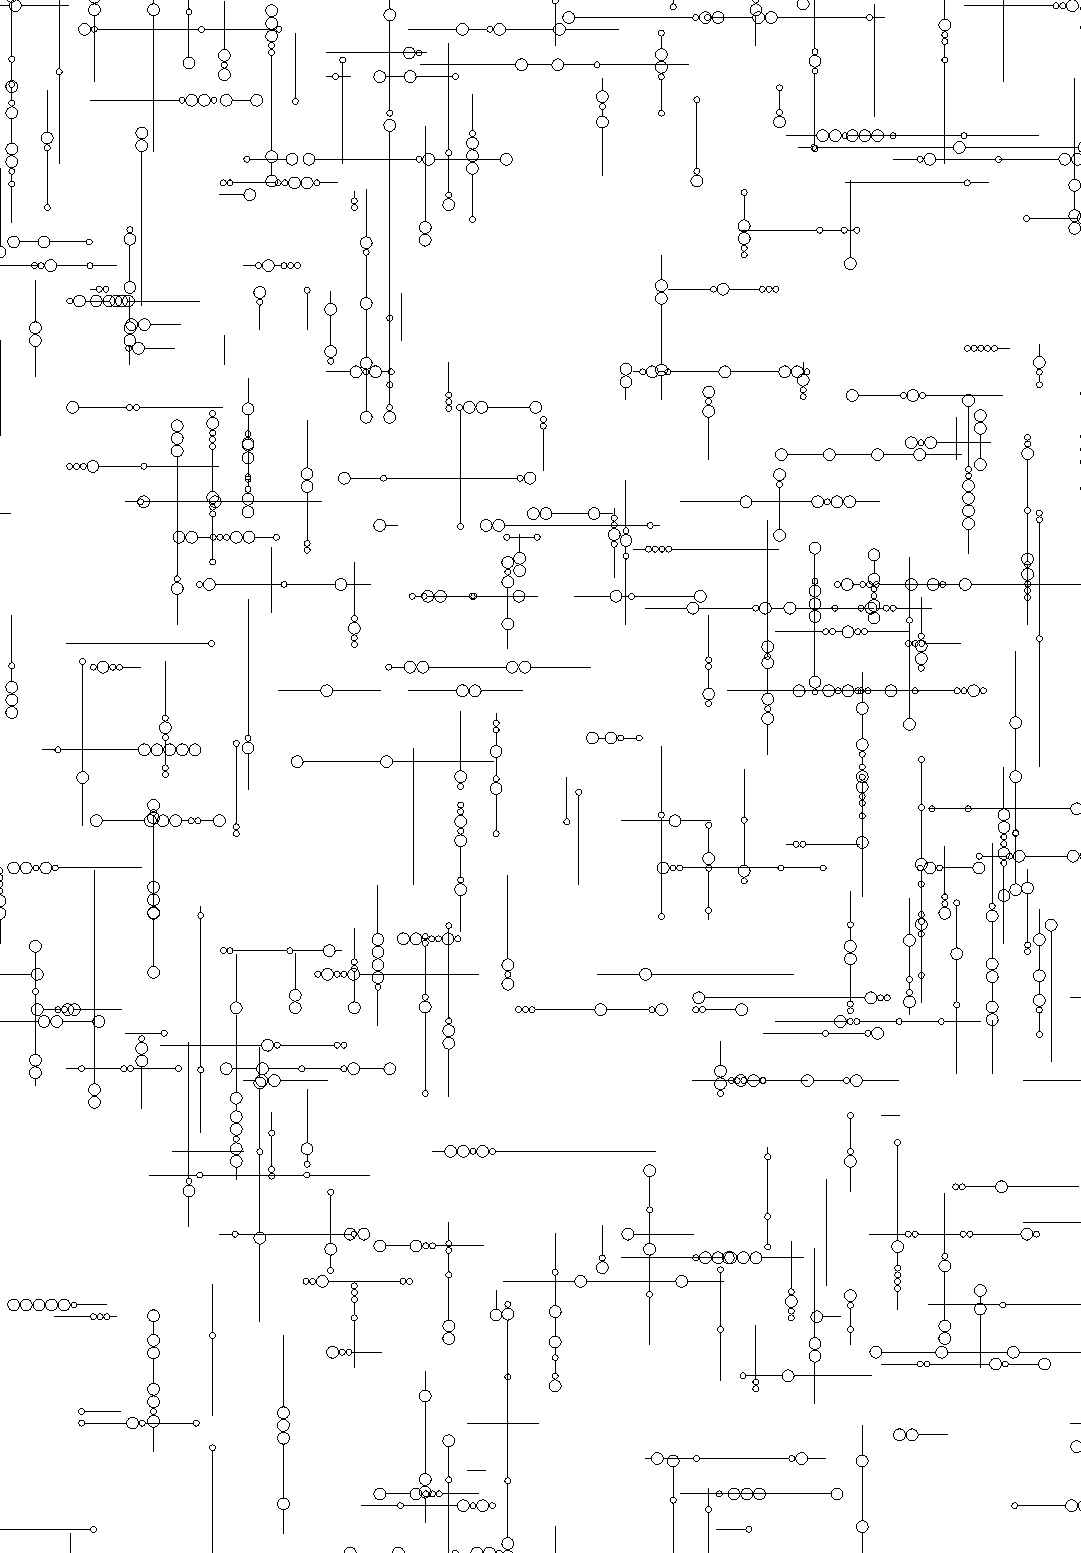
\includegraphics[scale=1.2]{patron.pdf}};
%%%%%%%%%%%%%%%%%%%%%%%%%%%%%%%%%%%%%%%%%%%%%%%%%%%%%%%%%%%%%%%%
%Rectas horizontales
\fill[shading=radial,inner color=colorAFILL,outer color=azuloscuro,draw=none,fill=none] ($(current page.south west)+(0,2cm)$) rectangle ($(current page.south east)+(0,2.25cm)$);
\fill[shading=radial,inner color=colorAFILL,outer color=azuloscuro,draw=none,fill=none] ($(current page.north west)+(0,-2cm)$) rectangle ($(current page.north east)+(0,-2.25cm)$);
%%%%%%%%%%%%%%%%%%%%%%%%%%%%%%%%%%%%%%%%%%%%%%%%%%%%%%%%%%%%%%%%
%Textos
\node[scale=5] at ($(current page.north)!0.382!(current page.south)$) (prac){\color{textoA}\selectfont \textsc{\shortstack[c]{\Practica\\\Grupo}}};
\node[anchor=south west,scale=5] at (prac.north west) {\selectfont \color{azul}\textbf{PDS-FPGAs}};
\node[anchor=east,scale=2] at ($(current page.south east)+(-0.5,8)$) {\color{textoB}\selectfont \shortstack[r]{\NombreUNO\\\NombreDOS}};
\end{tikzpicture}
%%%%%%%%%%%%%%%%%%%%%%%%%%%%%%%%%%%%%%%%%%%%%%%%%%%%%%%%%%%%%%%%
\else\ifnum\portada=2
\begin{tikzpicture}[overlay,remember picture]
\definecolor{fondo}{rgb}{0,0.1098,0.1333} %0 28 34
\definecolor{fondo2}{rgb}{0,0.0784,0.0941} %0 20 24
\fill[fill=fondo] (current page.north west) rectangle (current page.east);
\fill[fill=fondo2] (current page.west) rectangle (current page.south east);
\node[] at ($(current page.south)!1/1.6!(current page.north)$) {\includegraphics[width=\paperwidth]{prac1.png}};
\node[anchor=south] at ($(current page.south)+(0,0.1)$) (marca){
\includegraphics[scale=2]{marca_UPV_principal_color2.pdf}};
\fill[fill=fondo2,opacity=0.9] ($(marca.north west)$) rectangle (current page.south east);
\node[anchor=east,scale=2] at ($(current page.south)!0.236!(current page.north)+(8.5,0)$) {\color{white}\selectfont \shortstack[l]{\NombreUNO\\\NombreDOS}};
\end{tikzpicture}  
\else
\begin{tikzpicture}[overlay,remember picture]
\fill[fill=black] (current page.north west) rectangle (current page.east);
\fill[fill=black] (current page.west) rectangle (current page.south east);
\node[] at ($(current page.south)!1/1.6!(current page.north)$) {\includegraphics[width=\paperwidth]{prac1b.png}};
\node[anchor=south] at ($(current page.south)+(0,0.1)$) (marca){
\includegraphics[scale=2]{marca_UPV_principal_color2.pdf}};
\fill[fill=black,opacity=0.85] (marca.north west) rectangle (current page.south east);
\node[anchor=east,scale=2] at ($(current page.south)!0.236!(current page.north)+(8.5,0)$) {\color{white}\selectfont \shortstack[l]{\NombreUNO\\\NombreDOS}};
\end{tikzpicture}  
\fi\fi
\clearpage
\printmyminitoc




\section{Descripción del módulo}
%%%%%%%%%%%%%%%%%%%%%%%%%
\begin{enunciado}{}{}%
Breve explicación del bloque implementado indicando su funcionalidad y estructura interna. Se puede añadir (de apoyo a la explicación) una figura con el diagrama de bloques interno del modulo.
\end{enunciado}
%%%%%%%%%%%%%%%%%%%%%%%%%%%%%%%%%%%%%%%%%%%%%%%%%%%%%%%%%%%%%%%%%%%%%%%%%

%  .d8888b.   d888   % 
% d88P  Y88b d8888   % 
% 888    888   888   % 
% 888    888   888   % 
% 888    888   888   % 
% 888    888   888   % 
% Y88b  d88P   888   % 
%  "Y8888P"  8888888 % 
%%%%%%%%%%%%%%%%%%%%%%%%%

\section{Interfaz}
%%%%%%%%%%%%%%%%%%%%%%%%%
\begin{enunciado}{}{}%
Incluir las tablas en las que se definan el interfaz, sus formatos y sus parámetros. 
\end{enunciado}
%%%%%%%%%%%%%%%%%%%%%%%%%%%%%%%%%%%%%%%%%%%%%%%%%%%%%%%%%%%%%%%%%%%%%%%%%


% TABLA DEL INTERFAZ (4 COLUMNAS) %%%%%%%%%%%%%%%%%%%%%%%%
\input{tabla_4col}
% Definir los anchos de columna de la tabla
\def\colUNO{2cm}
\def\colDOS{1cm}
\def\colTRES{2.0cm}
\def\colCUATRO{10cm}

\begin{table}[H]
    \caption{Interfaz del módulo  DP\_mod}
    \label{tab:interfaz}
\gdef\cabecera{\fila{NOMBRE}{TIPO}{FORMATO}{DESCRIPCIÓN}}
\noindent\begin{mitabla}
% COMPLETAR FILAS. AÑADA LAS QUE NECESITE
\fila{}{}{}{} 
\fila{}{}{}{} 
\fila{}{}{}{} 
\fila{}{}{}{} 
\fila{}{}{}{} 
\fila{}{}{}{} 
\fila{}{}{}{} 
\fila{}{}{}{} 
\fila{}{}{}{} 
\fila{}{}{}{} 
\end{mitabla}
\end{table}

%  .d8888b.   .d8888b.  % 
% d88P  Y88b d88P  Y88b % 
% 888    888        888 % 
% 888    888      .d88P % 
% 888    888  .od888P"  % 
% 888    888 d88P"      % 
% Y88b  d88P 888"       % 
%  "Y8888P"  888888888  % 
%%%%%%%%%%%%%%%%%%%%%%%%%

\section{Recursos hardware}
%%%%%%%%%%%%%%%%%%%%%%%%%
\begin{enunciado}{}{}%
El objetivo de esta sección es que el alumno sea capaz de identificar si los recursos obtenidos en la implementación son coherentes con los esperables para el circuito realizado.

Se deberán incluir las siguientes partes: 
\begin{itemize}
\item \textbf{Estimación de recursos:} Un breve desglose de la estimación de recursos  del dispositivo FPGA que se requieren para implementar el módulo, indicando la cantidad de recursos asignados a cada bloque de su diseño. El resultado final se mostrará en una tabla. En esta práctica solo hay que indicar el número de LEs configurados en modo normal, LEs en modo aritmético, los multiplicadores de 18x18 bits, los FFs y memorias M9K. 

\item \textbf{Resultados obtenidos:} Una captura del resumen de recursos obtenidos con la herramienta Quartus tras la etapa de emplazamiento y rutado (Fitter), que se muestra en el report ``Resource Usage Summary''.  

\item \textbf{Análisis del resultado:} Un breve análisis de si los resultados obtenidos son coherentes con la estimación de recursos realizada. El análisis se realizará en base a la comparación entre lo estimado y obtenido en Quartus. Si hay muchas discrepancias con los recursos obtenidos, indicar razonadamente las causas de dicha discrepancia.
\end{itemize}

\end{enunciado}
%%%%%%%%%%%%%%%%%%%%%%%%%%%%%%%%%%%%%%%%%%%%%%%%%%%%%%%%%%%%%%%%%%%%%%%%%
\underline{\textbf{Estimación de recursos:}}

Los recursos hardware necesarios para implementar el bloque DP\_mod son los siguientes:
\begin{itemize}
\item \textbf{FFs:} 

\item \textbf{LEs normales:} 

\item \textbf{LEs aritméticos:} 

\item \textbf{Mults 18x18:} 

\item \textbf{M9Ks:} 
\end{itemize}

A continuación se muestra la tabla con el resumen de los recursos:

% TABLA RECURSOS (3 COLUMNAS) %%%%%%%%%%%%%%%%%%%%%%%%
\renewcommand{\fila}[2]{
\node[minimum height=2em,minimum width=1cm,anchor=north west,draw,outer sep=0pt,estilo] at (c0.south west) (c0) {\parbox{\colUNO}{\ifthenelse{\equal{\unexpanded{#1}}{}}{\ }{#1}}};
\node[minimum height=2em,minimum width=1cm,anchor=south west,draw,outer sep=0pt,estilo] at (c0.south east) (c1) {\parbox[c]{\colDOS}{\ifthenelse{\equal{\unexpanded{#2}}{}}{\ }{#2}}};}
% Definir los anchos de columna de la tabla
\def\colUNO{3cm}
\def\colDOS{5.5cm}
\def\colTRES{5.5cm}
%\def\colCUATRO{10cm}

\begin{table}[H]
\centering
    \caption{Recursos hardware}
    \label{tab:recursos_HW}
\gdef\cabecera{\fila{RECURSO}{NÚMERO OBTENIDO}}
\noindent\begin{mitabla}
% COMPLETAR FILAS
\fila{FFs}{}
\fila{LEs-normal}{}  
\fila{LEs-aritméticos}{}  
\fila{Mults 18x18}{}
\fila{M9Ks}{}
\end{mitabla}
\end{table}

\underline{\textbf{Resultados obtenidos:}}
% captura del resumen de recursos obtenidos con la herramienta Quartus tras la etapa de emplazamiento y rutado (Fitter), que se muestra en el report ``Resource Usage Summary''.

\underline{\textbf{Análisis del resultado:}}
% breve análisis de si los resultados obtenidos



%  .d8888b.   .d8888b.  % 
% d88P  Y88b d88P  Y88b % 
% 888    888      .d88P % 
% 888    888     8888"  % 
% 888    888      "Y8b. % 
% 888    888 888    888 % 
% Y88b  d88P Y88b  d88P % 
%  "Y8888P"   "Y8888P"  % 
%%%%%%%%%%%%%%%%%%%%%%%%% 

\section{Frecuencia de operación}
%%%%%%%%%%%%%%%%%%%%%%%%%
\begin{enunciado}{}{}

El objetivo de esta sección es que el alumno sea capaz de identificar  el camino crítico del módulo: el que condiciona su frecuencia máxima de funcionamiento.  
\begin{itemize}
    \item Obtenga la frecuencia máxima de operación del módulo implementado en el dispositivo usando la herramienta TimeQuest Timing Analyzer de Quartus e indique dónde se encuentra el camino crítico del circuito. En la tabla aparece un ejemplo de cómo debe indicar el camino crítico: siempre debe indicar desde qué registro se inicia y en qué registro finaliza.
    \item Realice un breve análisis de si es coherente que el camino crítico sea el obtenido por la herramienta TimeQuest o si cree que debería estar en otra parte del circuito.
\end{itemize}

Para realizar el análisis debe tener en cuenta que el camino crítico es el camino entre dos registros con mayor retardo y los retardos en el dispositivo FPGA los producen la lógica combinacional (LUTs) y el rutado. Si un camino tiene más lógica combinacional (más profundidad de lógica: la señal pasa por más LUTs en cascada) generará más retardo debido a la lógica. Si al emplazarse los recursos de un camino concreto (registros y lógica) más separados dentro del chip, esto producirá más retardo por rutado.  

\end{enunciado}

% TABLA DEL Fmax (2 COLUMNAS) %%%%%%%%%%%%%%%%%%%%%%%%
\renewcommand{\fila}[2]{
\node[minimum height=2em,minimum width=1cm,anchor=north west,draw,outer sep=0pt,estilo] at (c0.south west) (c0) {\parbox{\colUNO}{\ifthenelse{\equal{\unexpanded{#1}}{}}{\ }{#1}}};
\node[minimum height=2em,minimum width=1cm,anchor=south west,draw,outer sep=0pt,estilo] at (c0.south east) (c1) {\parbox[c]{\colDOS}{\ifthenelse{\equal{\unexpanded{#2}}{}}{\ }{#2}}};}
% Definir los anchos de columna de la tabla
\def\colUNO{3cm}
\def\colDOS{12cm}
%\def\colTRES{2.0cm}
%\def\colCUATRO{10cm}

\begin{table}[H]
    \caption{Frecuencia de reloj y camino crítico}
    \label{tab:frec_clk}
\gdef\cabecera{\fila{$f_{clk} $ (MHz)}{CAMINO CRÍTICO}}
\noindent\begin{mitabla}
% COMPLETAR FILAS
\fila{}{} 
\end{mitabla}
\end{table}


\underline{\textbf{Análisis del resultado:}}

El camino crítico obtenido es coherente por estas razones ...

%%%%%%%%%%%%%%%%%%%%%%%%%%%%%%%%%%%%%%%%%%%%%%%%%%%%%%%%%%%%%%%%%%%%%%%%%


%  .d8888b.      d8888  % 
% d88P  Y88b    d8P888  % 
% 888    888   d8P 888  % 
% 888    888  d8P  888  % 
% 888    888 d88   888  % 
% 888    888 8888888888 % 
% Y88b  d88P       888  % 
%  "Y8888P"        888  % 
%%%%%%%%%%%%%%%%%%%%%%%%%

\section{Verificación}
%%%%%%%%%%%%%%%%%%%%%%%%%
\begin{enunciado}{}{}%
Resultados de la verificación al excitarlo con diferentes entradas para demostrar su completo funcionamiento. Solo se incluirá:
\begin{itemize}
    \item La lista de las pruebas realizadas, que debe coincidir con los casos de test que se hayan configurado en el script de simulación de Matlab.
    \item Las capturas de las formas de onda y el resumen (mostrado en la consola de Modelsim) de la simulación realizada de un máximo de 2 casos, mostrando claramente el comportamiento del circuito y que no existen errores al compararlo con el modelo de Simulink.
\end{itemize}

\end{enunciado}
%%%%%%%%%%%%%%%%%%%%%%%%%%%%%%%%%%%%%%%%%%%%%%%%%%%%%%%%%%%%%%%%%%%%%%%%%

El módulo ha funcionado correctamente. Su funcionamiento se ha verificado con las siguientes pruebas:
\begin{enumerate}
    \item 
    \item 
    \item
\end{enumerate}

A continuación, se describen dos de los escenarios de test enumerados anteriormente:
\subsection{Caso 1: }

%   \begin{center}
%   \includegraphics[width=19cm]{XXXXX.png}
%   \end{center}

\subsection{Caso 2}

%  .d8888b.  888888888  % 
% d88P  Y88b 888        % 
% 888    888 888        % 
% 888    888 8888888b.  % 
% 888    888      "Y88b % 
% 888    888        888 % 
% Y88b  d88P Y88b  d88P % 
%  "Y8888P"   "Y8888P"  % 
%%%%%%%%%%%%%%%%%%%%%%%%%

%%%%%%%%%%%%%%%%%%%%%%%%%%%%%%%%%%%%%%%%%%%%%%%%%%%%%%%%%%%%%%%%%%%%%%%%%

\section{Conclusiones}
%%%%%%%%%%%%%%%%%%%%%%%%%
\begin{enunciado}{}{}%
Conclusiones de la práctica. Valore el grado de cumplimiento de los objetivos de la práctica y el grado de coherencia entre los valores estimados de área y los obtenidos, así como de la frecuencia máxima de funcionamiento.  
\end{enunciado}


%%%%%%%%%%%%%%%%%%%%%%%%%%%%%%%%%%%%%%%%%%%%%%%%%%%%%%%%%%%%%%%%%%%%%%%%%

%  .d8888b.   .d8888b.  % 
% d88P  Y88b d88P  Y88b % 
% 888    888 888        % 
% 888    888 888d888b.  % 
% 888    888 888P "Y88b % 
% 888    888 888    888 % 
% Y88b  d88P Y88b  d88P % 
%  "Y8888P"   "Y8888P"  % 
%%%%%%%%%%%%%%%%%%%%%%%%%

\section{Ficheros entregados}
%%%%%%%%%%%%%%%%%%%%%%%%%
\begin{enunciado}{}{}%
Lea el documento \href{https://gised.webs.upv.es/pds_fpga/PDS_FPGA_practicas.pdf} {desarrollo y entrega de prácticas}  e indique cómo se han nombrado los ficheros que se indican en la tabla.  En esta práctica esta tabla está por completar, para que sirva de referencia para las siguientes prácticas.

\end{enunciado}
%%%%%%%%%%%%%%%%%%%%%%%%%%%%%%%%%%%%%%%%%%%%%%%%%%%%%%%%%%%%%%%%%%%%%%%%%

Los autores de la memoria confirman que han entregado los ficheros siguientes, siguiendo las pautas indicadas:
% TABLA DE PARÁMTROS (2 COLUMNAS) %%%%%%%%%%%%%%%%%%%%%%%%
\renewcommand{\fila}[2]{
\node[minimum height=2em,minimum width=1cm,anchor=north west,draw,outer sep=0pt,estilo] at (c0.south west) (c0) {\parbox{\colUNO}{\ifthenelse{\equal{\unexpanded{#1}}{}}{\ }{#1}}};
\node[minimum height=2em,minimum width=1cm,anchor=south west,draw,outer sep=0pt,estilo] at (c0.south east) (c1) {\parbox[c]{\colDOS}{\ifthenelse{\equal{\unexpanded{#2}}{}}{\ }{#2}}};}
% Definir los anchos de columna de la tabla
\def\colUNO{10cm}
\def\colDOS{4cm}

\begin{table}[H]
    \centering
    %\caption{Entregables de la práctica E1}
    \label{tab:entregables}
\gdef\cabecera{\fila{FICHERO}{NOMBRE}}
\noindent\begin{mitabla}
% COMPLETAR FILAS. AÑADA LAS QUE NECESITE
\fila{Memoria de prácticas}{Memoria\_P2\_Gx.pdf}
\fila{Entrega de los ficheros de prácticas}{Proy\_sim\_P2\_Gx.zip}
\fila{Proyecto Modelsim}{}
\fila{Fichero .do}{dp\_mod\_tsb.do}
\fila{Fichero .tcl}{dp\_mod\_tsb.tcl}
\fila{Proyecto Quartus}{}
\end{mitabla}
\end{table}

%  .d8888b.  8888888888 % 
% d88P  Y88b       d88P % 
% 888    888      d88P  % 
% 888    888     d88P   % 
% 888    888  88888888  % 
% 888    888   d88P     % 
% Y88b  d88P  d88P      % 
%  "Y8888P"  d88P       % 
%%%%%%%%%%%%%%%%%%%%%%%%%

\section{ANEXO 1: Código HDL del módulo dp\_mod}

%%%%%%%%%%%%%%%%%%%%%%%%%
\begin{enunciado}{}{}%
Incluir un esquema de la división en bloques realizada y el código Verilog de los módulos de la práctica. El código debe ser legible, ordenado, bien tabulado y comentado. El código debe seguir las pautas indicadas en el documento  \href{https://gised.webs.upv.es/pds_fpga/PDS_FPGA_practicas.pdf} {desarrollo y entrega de prácticas}. 
\end{enunciado}
%%%%%%%%%%%%%%%%%%%%%%%%%%%%%%%%%%%%%%%%%%%%%%%%%%%%%%%%%%%%%%%%%%%%%%%%%

\begin{minted}[fontsize=\footnotesize,obeytabs=true,tabsize=2]{verilog}
module dp_mod
	(
	input signed [15:0] id_data,	// S[16,15] 
	input [23:0] id_frec_por,		// U[24,24]
	input [15:0] id_im_am,			// U[16,15]
	input [15:0] id_im_fm,			// U[16,16]
	input ic_fm_am, 				// Control modo fm/am
	input ic_rst,					// rst sincrono activo a 1
	input ic_val_data,				
	input clk,
	output signed [15:0] od_data,	// S[16,15]
	output oc_val_data
	);
	
/* DECLARACIONES ----------------------- */

/* DESCRIPCION ------------------------- */	

/* ASIGNACION SALIDAS ------------------ */

endmodule 
\end{minted}



%  .d8888b.   .d8888b.  % 
% d88P  Y88b d88P  Y88b % 
% 888    888 Y88b. d88P % 
% 888    888  "Y88888"  % 
% 888    888 .d8P""Y8b. % 
% 888    888 888    888 % 
% Y88b  d88P Y88b  d88P % 
%  "Y8888P"   "Y8888P"  % 
%%%%%%%%%%%%%%%%%%%%%%%%%


\section{ANEXO 2: Código HDL del banco de pruebas dp\_mod\_tsb}
%%%%%%%%%%%%%%%%%%%%%%%%%
\begin{enunciado}{}{}%
Incluir el código Verilog del banco de pruebas realizado.
\end{enunciado}
%%%%%%%%%%%%%%%%%%%%%%%%%%%%%%%%%%%%%%%%%%%%%%%%%%%%%%%%%%%%%%%%%%%%%%%%%

\begin{minted}[fontsize=\footnotesize,obeytabs=true,tabsize=2]{verilog}
`timescale 1ns/1ps

module dp_mod_tsb();


endmodule 


\end{minted}

%  .d8888b.   .d8888b.  % 
% d88P  Y88b d88P  Y88b % 
% 888    888 888    888 % 
% 888    888 Y88b. d888 % 
% 888    888  "Y888P888 % 
% 888    888        888 % 
% Y88b  d88P Y88b  d88P % 
%  "Y8888P"   "Y8888P"  % 
%%%%%%%%%%%%%%%%%%%%%%%%%



\end{document}